\section{simulación de orbitas en Kerr}
De manera genérica para construir una simulación de las geodésicas en Kerr, consideremos los parámetros del agujero negro como lo son $a$ y $m$. Estos parámetros determinan la forma de la métrica y, por lo tanto, las trayectorias de las partículas que orbitan el agujero negro, y se consideran fijos.

La simulación numérica se hizo en python con las librerías de SciPy y NumPy para resolver las ecuaciones \ref{eq:kerr_geodesics_mino}, posteriormente se utilizó la librería Matplotlib para la visualización de las trayectorias.


\begin{lstlisting}[language=Python, caption= {Este es el código genérico para la simulación de geodésicas en el espacio-tiempo de Kerr, se fijaron valores para las constantes $E$ y $L_z$, posiciones iniciales para $r$, $\theta$, $\phi$ y $t$. Además se uso la constante de masa $\mu$ a 1, asi como también $c$ a 1.Posteriormente se puede usar Matplotlib para ver las trayectorias, se puede encontar el codigo completo en los anexos \ref{chap:programa_geodesicas}.}]

import numpy as np
from scipy.integrate import solve_ivp
import matplotlib.pyplot as plt

# --- Variables Globales para el Manejo de Puntos de Inflexión ---
# Guardan el signo de la velocidad para saber si la partícula va hacia adentro/afuera
# o hacia arriba/abajo.
sign_r = 1.0  # Empezamos moviéndonos hacia afuera
sign_theta = 1.0 # Empezamos moviéndonos hacia el polo norte

# Guardan el valor de la derivada anterior para ayudar a detectar el cambio de signo.
dr_dtau_prev = 0.0
dtheta_dtau_prev = 0.0


# Constantes del agujero negro
a = 0.9
m = 1.0
c = 1.0

# Constantes de la geodésica
# Estas se calclulan por separado
# Constantes de movimiento para una órbita inclinada y en precesión
E = 0.95     # Energía 
Lz = 3.0     # Momento angular axial
Q = 15.0     # Constante de Carter (alta para una gran inclinación)
mu = 1.0     # Masa de la partícula (1 para masiva, 0 para fotón)

# Condiciones iniciales [r0, theta0, phi0, t0]
r0 = 6.0*m
theta0 = np.pi / 3  # Inclinación inicial de 60 grados respecto al ecuador
phi0 = 0.0
t0 = 0.0
y0 = [r0, theta0, phi0, t0]


tau_max = 100
tau_span = [0, tau_max]

def kerr_geodesics(tau, y, m, a, E, Lz, Q):
    """
    Define el sistema de EDOs para las geodésicas de Kerr en tiempo Mino (tau).
    El vector de estado es y = [r, theta, phi, t].
    """
    global sign_r, sign_theta, dr_dtau_prev, dtheta_dtau_prev
    r, theta, phi, t = y

    # Términos auxiliares de la métrica
    Delta = r**2 - 2 * m * r + a**2


    Rr = ((r**2 + a**2) * (E/c) - a * Lz)**2 - Delta * ((mu * c * r)**2 + (Lz - a * (E/c))**2 + Q)

    # El término np.sin(theta)**2 + 1e-9 evita la división por cero en los polos.
    Th = Q - np.cos(theta)**2 * (Lz**2 / (np.sin(theta)**2 + 1e-9)+a**2 * ((mu* c)**2 - (E/c)**2))

    # Se truncan a cero valores negativos pequeños que puedan surgir de errores de precisión.
    Rr = max(Rr, 0.0)
    Th = max(Th, 0.0)

    # Detección y manejo simple de puntos de inflexión (turning points)
    # Si el potencial es casi cero y la velocidad anterior era mayor, invertimos la dirección.
    if Rr < 1e-7 and dr_dtau_prev**2 > Rr:
        sign_r *= -1
    if Th < 1e-7 and dtheta_dtau_prev**2 > Th:
        sign_theta *= -1

    # Derivadas con respecto al tiempo Mino (tau)
    dr_dtau = sign_r * np.sqrt(Rr)
    dtheta_dtau = sign_theta * np.sqrt(Th)

    # Actualizamos los valores de las derivadas para la siguiente iteración
    dr_dtau_prev = dr_dtau
    dtheta_dtau_prev = dtheta_dtau

    dphi_dtau = (Lz / (np.sin(theta)**2 + 1e-9) - a * (E/c)) + (a *((r**2 + a**2) * (E/c) - a * Lz) / Delta)

    dt_dtau = - a * (a * (E/c) * np.sin(theta)**2 - Lz) + ((r**2 + a**2) * ((r**2 + a**2) * (E/c) - a * Lz) / Delta)

    return [dr_dtau, dtheta_dtau, dphi_dtau, dt_dtau]

print("Iniciando la integración numérica...")

# Genera 2000 puntos espaciados uniformemente para una curva suave.
t_eval_points = np.linspace(tau_span[0], tau_span[1], 2000) 

# Llamada al solver de EDOs de SciPy
sol = solve_ivp(
    fun=kerr_geodesics,
    t_span=tau_span,
    y0=y0,
    args=(m, a, E, Lz, Q),
    method='Radau',      # Un método robusto para este tipo de problemas
    dense_output=True,   # Permite obtener una solución continua y suave
    rtol=1e-8,           # Tolerancia relativa para alta precisión
    atol=1e-8,           # Tolerancia absoluta
    t_eval=t_eval_points # Puntos donde se evalúa la solución
)


print("Integración completada con éxito.")


# Extraer los resultados de la solución
r, theta, phi, t = sol.y
\end{lstlisting}

En este ejemplo se propuso las cantidades $E$, $L_z$ y $\mathcal{Q}$, en un flujo de trabajo realista se propone el punto de partida  $(r_0, \theta_0, \phi_0, t_0)$, para posteriormente proponer los valores de $E$, $L_z$ y $\mathcal{Q}$ para la situación que se desee analizar (y si se desea calcular las velocidades o momentos iniciales), o bien a partir de las condiciones iniciales de posición y velocidad (o momento) de la partícula en la geodésica calcular el valor de estas constantes.

\begin{figure}[H]
    \begin{subfigure}{0.5\textwidth}
        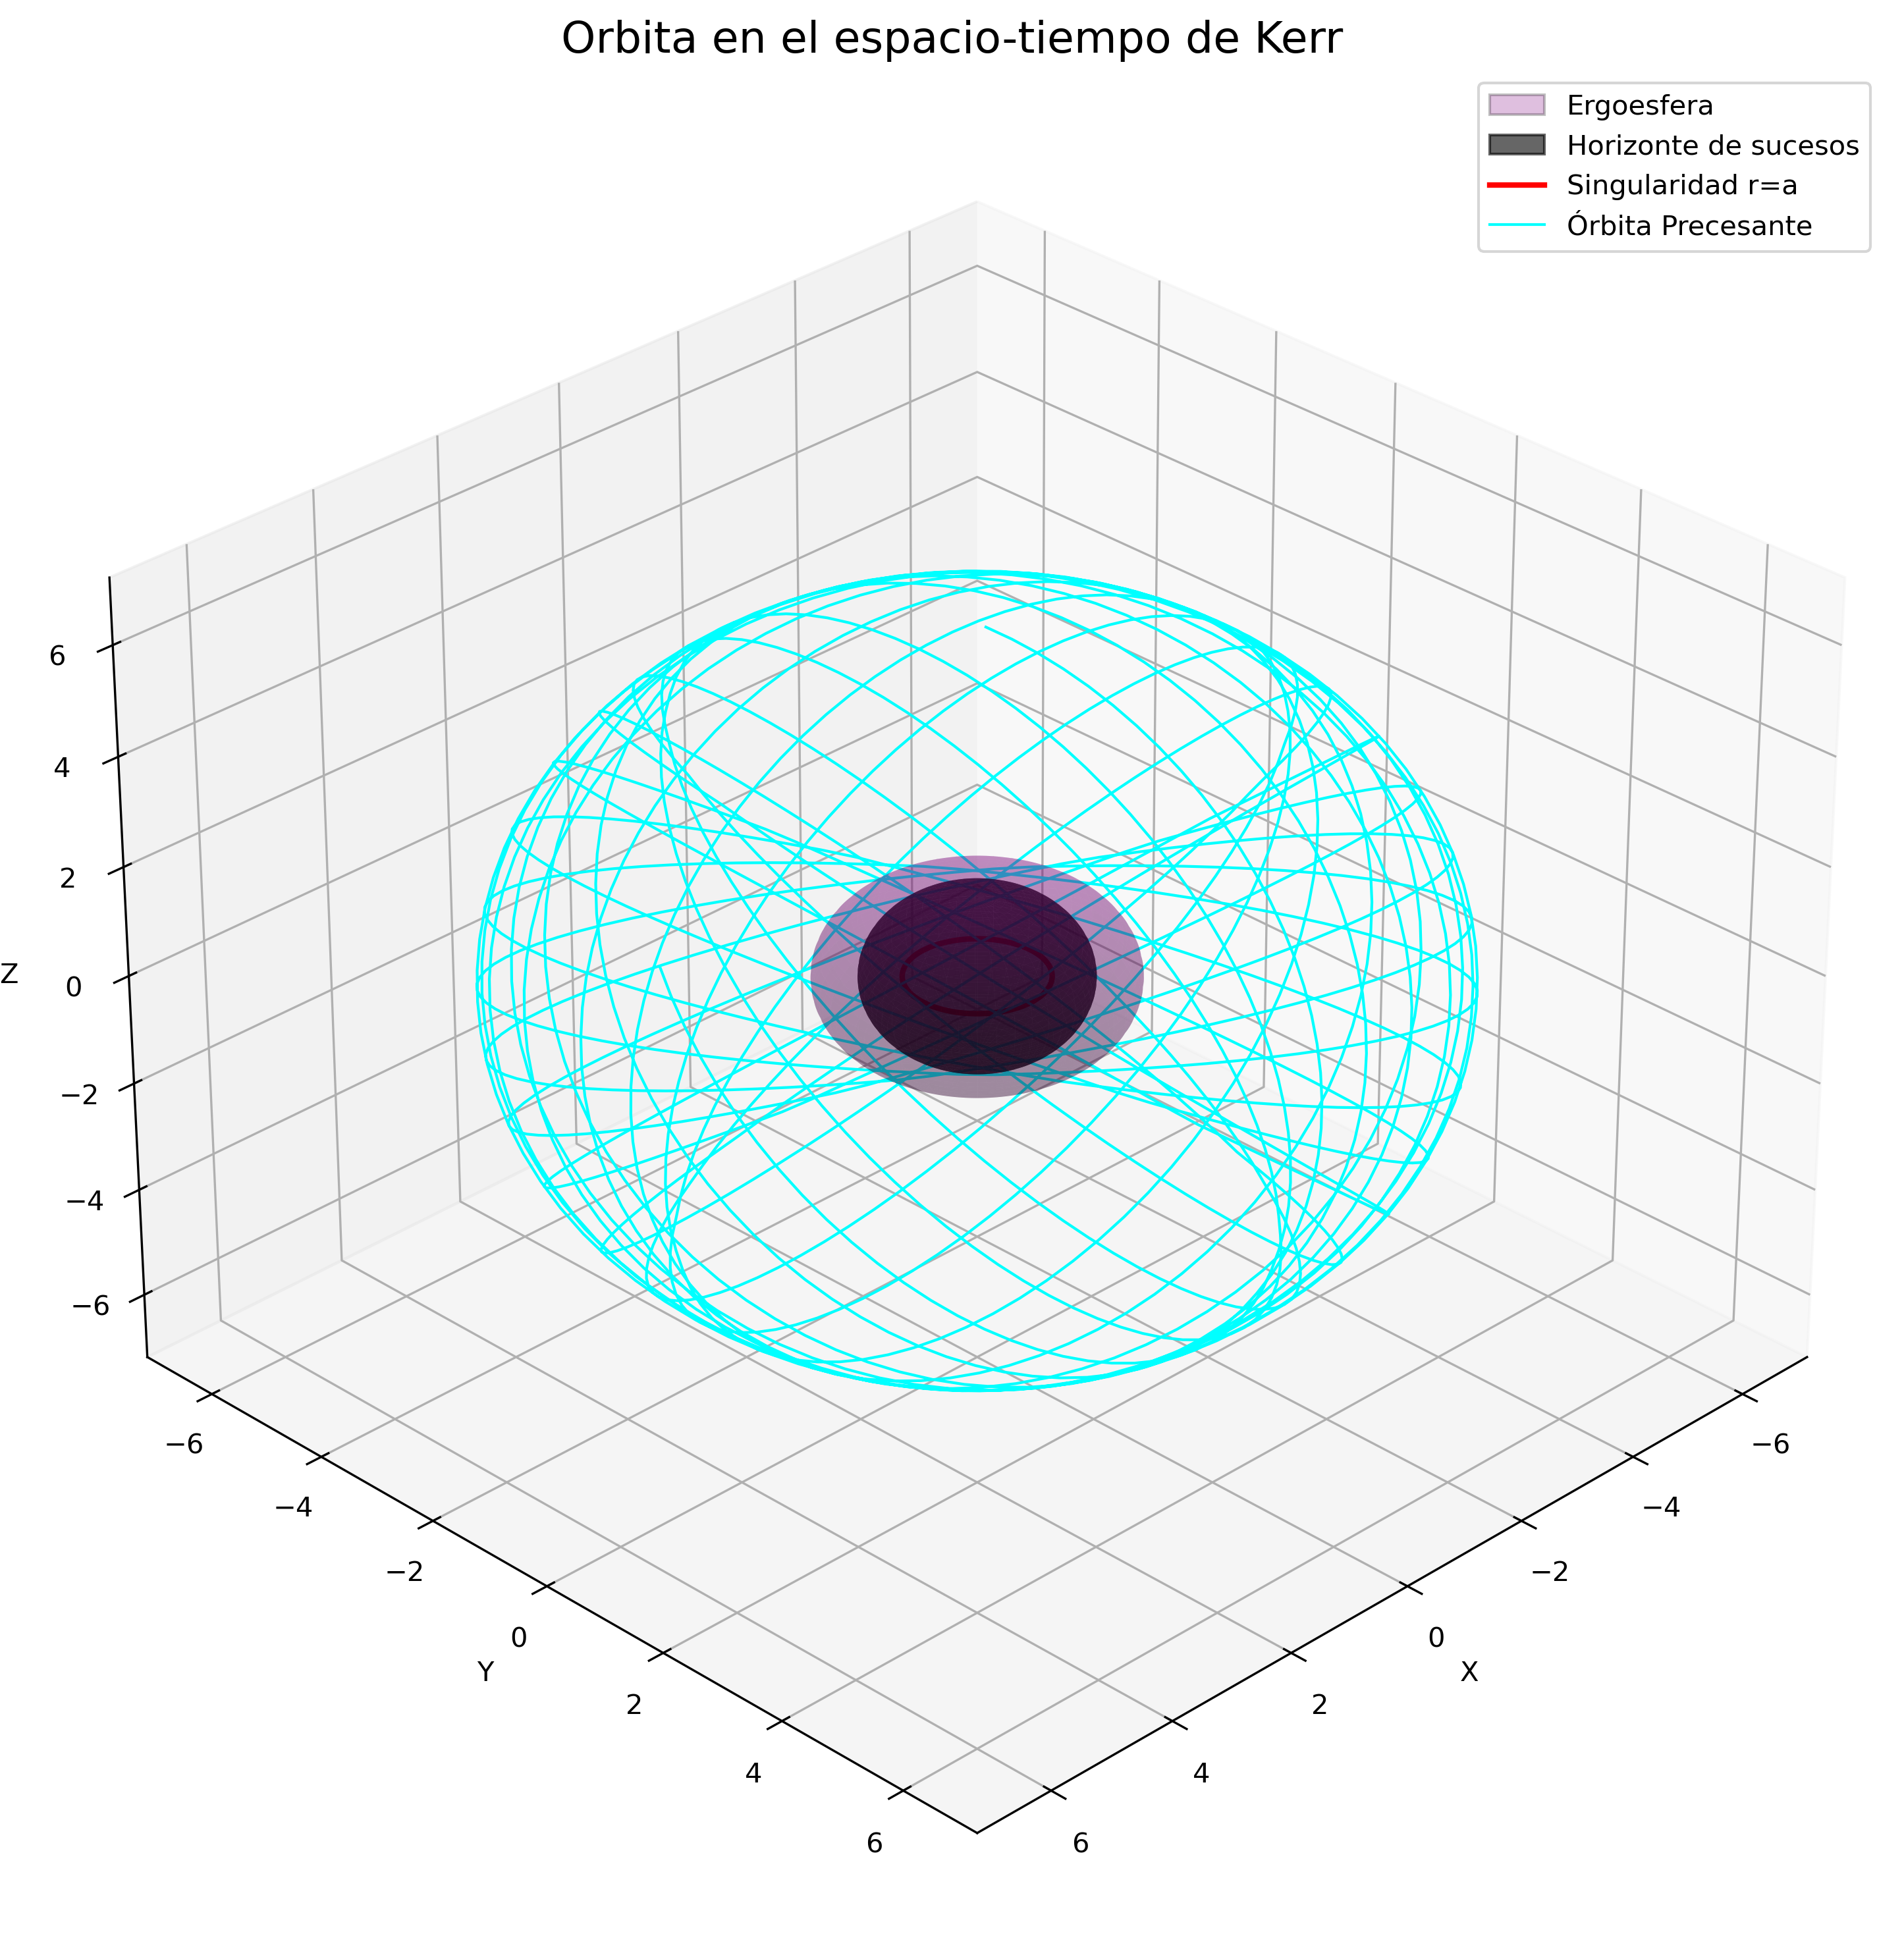
\includegraphics[width=0.9\linewidth, height=6cm]{AgujerosNegros/kerr/geodesics_plots/Geodesica1.png}
        \caption{Trayectoria de la partícula en el espacio-tiempo de Kerr}
    \end{subfigure}
    \begin{subfigure}{0.5\textwidth}
        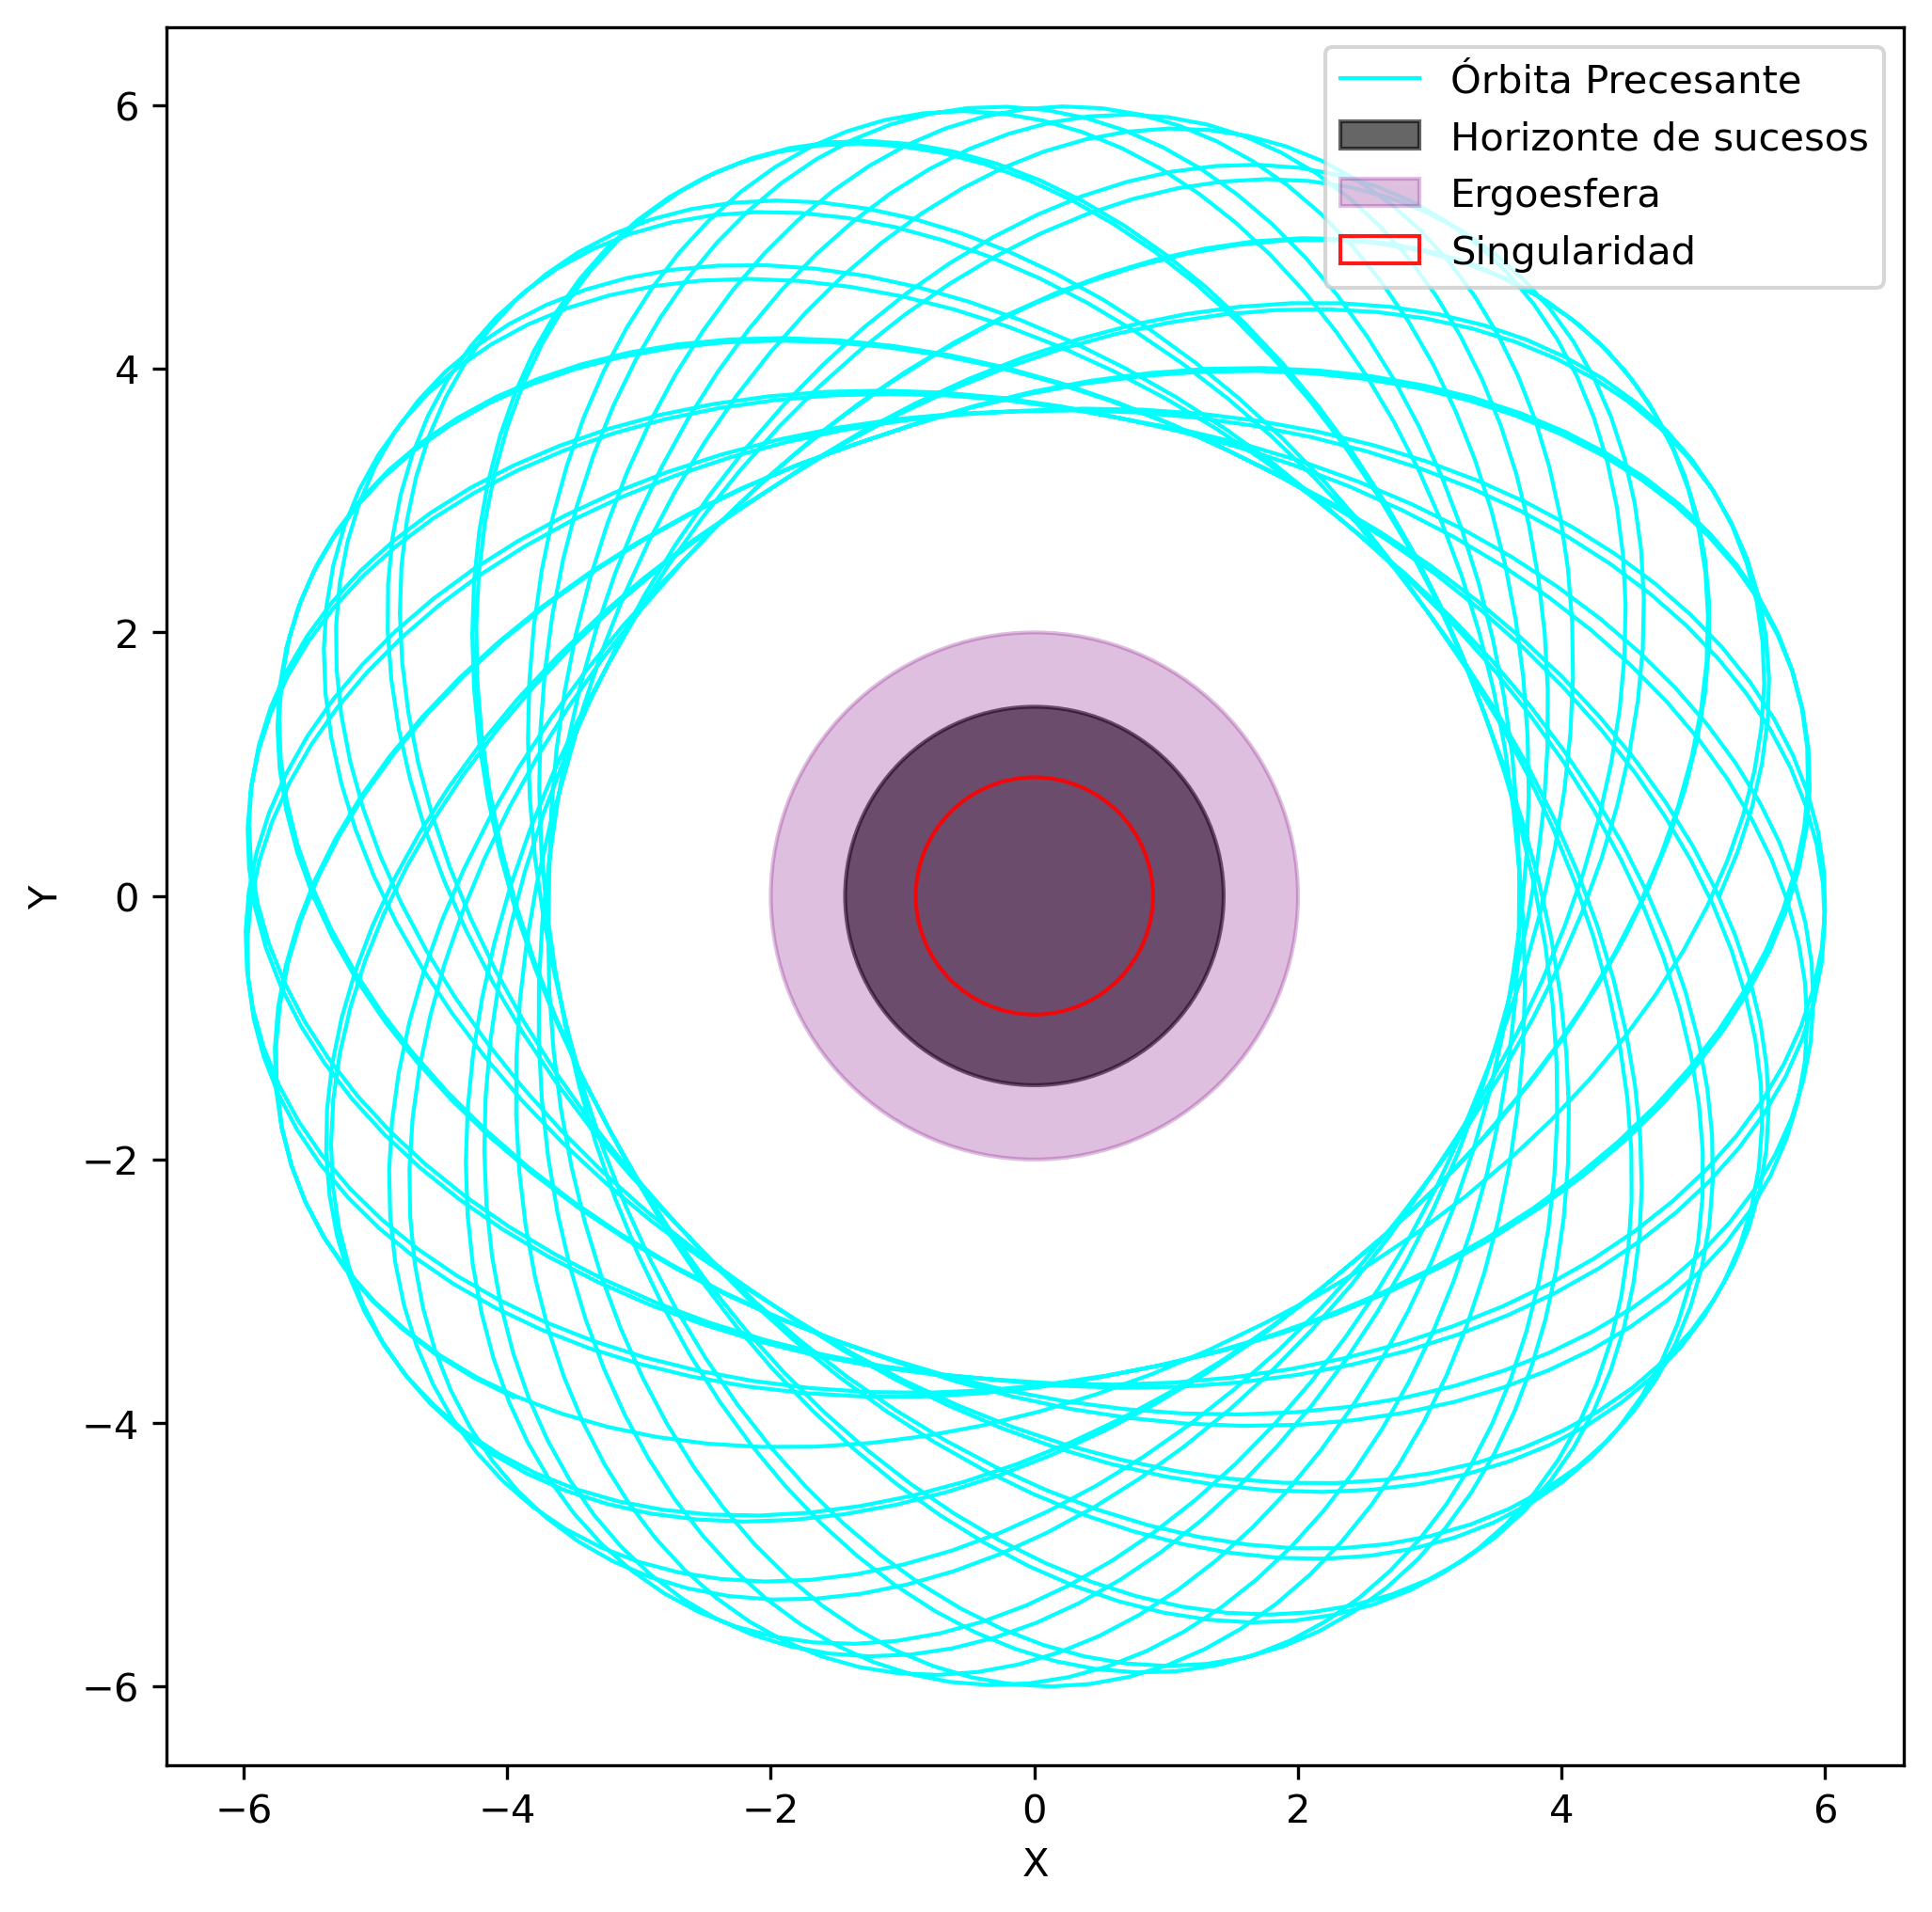
\includegraphics[width=0.9\linewidth, height=6cm]{AgujerosNegros/kerr/geodesics_plots/Geodesica1_planoxy.png}
        \caption{Trayectoria de la partícula en el plano $x-y$}
    \end{subfigure}
    \caption{Trayectoria de la partícula en el espacio-tiempo de Kerr con parámetros $a=0.9$, $m=1$, $E=0.95$, $L_z=3$ y $\mathcal{Q}=15$. La partícula inicia en $r_0=6m$, $\theta_0=\pi/3$, $\phi_0=0$ y $t_0=0$ y con $c = 1$. Se observa una órbita inclinada con precesión alrededor del agujero negro.}
\end{figure}

